\documentclass[conference]{IEEEtran}
\IEEEoverridecommandlockouts
% The preceding line is only needed to identify funding in the first footnote. If that is unneeded, please comment it out.
\usepackage{cite}
\usepackage{amsmath,amssymb,amsfonts}
\usepackage{algorithmic}
\usepackage{graphicx}
\usepackage{textcomp}
\usepackage{xcolor}
\def\BibTeX{{\rm B\kern-.05em{\sc i\kern-.025em b}\kern-.08em
    T\kern-.1667em\lower.7ex\hbox{E}\kern-.125emX}}
\begin{document}

\title{Conference Paper Title\\
\thanks{Identify applicable funding agency here. If none, delete this.}
}

\author{\IEEEauthorblockN{1\textsuperscript{st} Given Name Surname}
\IEEEauthorblockA{\textit{dept. name of organization (of Aff.)} \\
\textit{name of organization (of Aff.)}\\
City, Country \\
email address or ORCID}
\and
\IEEEauthorblockN{2\textsuperscript{nd} Given Name Surname}
\IEEEauthorblockA{\textit{dept. name of organization (of Aff.)} \\
\textit{name of organization (of Aff.)}\\
City, Country \\
email address or ORCID}
\and
\IEEEauthorblockN{3\textsuperscript{rd} Given Name Surname}
\IEEEauthorblockA{\textit{dept. name of organization (of Aff.)} \\
\textit{name of organization (of Aff.)}\\
City, Country \\
email address or ORCID}
\and
\IEEEauthorblockN{4\textsuperscript{th} Given Name Surname}
\IEEEauthorblockA{\textit{dept. name of organization (of Aff.)} \\
\textit{name of organization (of Aff.)}\\
City, Country \\
email address or ORCID}
\and
\IEEEauthorblockN{5\textsuperscript{th} Given Name Surname}
\IEEEauthorblockA{\textit{dept. name of organization (of Aff.)} \\
\textit{name of organization (of Aff.)}\\
City, Country \\
email address or ORCID}
\and
\IEEEauthorblockN{5\textsuperscript{th} Given Name Surname}
\IEEEauthorblockA{\textit{dept. name of organization (of Aff.)} \\
\textit{name of organization (of Aff.)}\\
City, Country \\
email address or ORCID}
}

\maketitle

\begin{abstract}
Citation networks are graphical networks composed of publications as nodes and citations as edges. 
They offer a unique look into scientific collaboration and the flow of knowledge within academia. 
In this paper, we examine the history of machine learning hardware papers through the lens of citation 
networks and construct GNN models for node classification and link prediction for our custom machine 
learning hardware dataset as well as existing datasets in software engineering and machine learning. 
We utilize existing citation graphs as well as curate our own dataset from the Web of Science database 
to show that node classification and link prediction are effective on a new network of machine learning 
hardware papers.
\end{abstract}

% \begin{IEEEkeywords}
% component, formatting, style, styling, insert
% \end{IEEEkeywords}

\section{Introduction and Motivation}
Inspired by the recent advent of graphical neural networks (GNNs), this project explores their potential to classify academic networks. 
Given any individual publication or author, GNNs could predict their relation to the remainder of the network, 
useful for understanding the relationships between academic fields, authors, institutions, and more. This opens the door to 
opportunities for classifying papers in fields with minimal representation in existing citation networks or predicting links 
between papers, potentially applicable to discovering inspiring papers related to an author's past work, 
among other capabilities. \par

In particular, machine learning hardware is a new field that has skyrocketed from the recent popularity of machine learning. 
Due to the compute-intensive nature of this field, plenty of research exists in the hardware infrastructure to support these 
computing loads. We utilize GNNs for node classification and link prediction to explore existing datasets and comment on the 
new corpus of machine learning hardware papers. The main challenges are processing data for useful representations of the network 
and data interpretation on the created GNNs to comment on the field of machine learning hardware. \par

\section{Previous Work}
There have been many previous explorations of citation networks using the datasets Cora, Citeseer, and PubMed Diabetes. 
In these citation networks, in particular, node classification and link prediction have been heavily explored. 
In Optimization of Graph Neural Networks with Natural Gradient Descent, Izadi et al improve on traditional optimization 
algorithms such as ADAM and stochastic gradient descent (SGD), producing a superior accuracy (90.16±0.59\%) 
by utilizing a proposed method inspired by natural gradient descent [1]. This paper achieved the highest accuracy across 
71 different papers done on node classification of the Cora dataset.  \par

Those that explored link prediction in the Cora and Citeseer datasets have achieved great results as well. 
In ‘NESS: Node Embeddings from Static SubGraphs,’ Ucar proposed splitting up the graph into multiple subgraphs 
that do not have overlapping edges in between subgraphs, using each graph to train and obtain node representations, 
then aggregating the results to obtain predictions [2]. Using this, he was able to obtain state-of-the-art accuracy results, 
achieving 98.94±0.1\% on Citeseer and 96.81±0.6\% on Cora. In ‘Neural Link Prediction with Walk Pooling,’ L. 
Pan et al proposed a GNN architecture that adds attention mechanisms to GNNs, achieving an accuracy of 89.59±1.58\% [3]. 
These past studies show the efficacy of GNNs on academic publications for node classification and link prediction, and, 
since these accuracies were certainly impressive, we hope to use these networks as a baseline to examine the key features 
of different datasets and extract information to create a similar dataset about the subject of machine learning hardware.  \par

\section{Approach}

Two preconstructed datasets, Cora and CiteSeer, are large datasets of scientific machine learning papers. 
Each dataset contains papers from before 2008, with citations to other papers in the database as well as the 
vocabulary used. The nodes of the graph are the papers themselves, with topics and vocabulary as individual features, 
while the directed links are citations to other papers. Cora classifies each publication into one of seven categories: 
Theory, Reinforcement Learning, Genetic Algorithms, Neural Networks, Probabilistic Methods, Case Based, and Rule Learning. 
On the other hand, Citeseer classifies each publication into one of six categories: Agents, Artificial Intelligence, Database, 
Human Computer Interaction, Machine Learning, and Information Retrieval. \par

Meanwhile, PubMed is a database of diabetes publications that is classified into one of three classes [4]. As such, this 
dataset is similar to both Cora and CiteSeer, though it further explores the efficacy of GNNs on datasets outside of 
machine learning. This performance of this dataset can further validate parameters potentially affecting accuracies, 
such as edge count, classes, or path length,  in addition to explaining differences in different fields of publications. \par

Web of Science (WoS) is an online database of publication citations and information [5]. 
This online database created by Clarivate can be queried by genre and shows identifying information such as titles, 
references, and specific citations. As such, we can utilize the WoS dataset to address the goal of exploring additional 
datasets in machine learning hardware. Specifically, by downloading papers by (exclusive) topic, 
we can create a dataset representative of the field of machine learning and compare the performance of our dataset 
against GNNs alongside other common datasets to analyze its efficacy on these models and its viability as a dataset 
in an academic setting. Using this popular database, we query their dataset of publications for four categories: 
Machine Learning on the Edge, Neuromorphic Computing, Spiking Neural Networks, and Machine Learning Accelerator. 
In using the Web of Science database, we assume that the papers are representative of their assigned class and 
distinct from related classes. In this regard, the dataset that we curate is unique from other citation networks 
in that it will hold distinct characteristics and be of machine learning hardware, providing insight into the 
structure and nature of the machine learning hardware citation network. \par

Beginning with the provided models like Deep Graph Library, we take inspiration from existing methods, 
such as preprocessing methods discussed by the Semantic Scholar Academic Graph [6]. By constructing our 
datasets of publications, we will examine model characteristics of varying types of publication networks. 
We also explored other datasets to improve the diversity of our datasets. The  Microsoft Open Academic Graph [7], 
a large academic graph dataset, shows a promising example of dataset scale, though it has differences in 
features, scaling, and overlapping that can interfere with providing information about any one academic field. 
Here, the data set uses a variety of data types for the nodes, like publications, authors, and venues, with 
the links between each denoting a correlation. \par 

Following the specified approach to our project goals, the main tasks of our project are as follows. 
First, we will apply the necessary pre-processing techniques to each dataset for model compatibility. 
Then, we will create a GNN model using each dataset that accurately predicts paper topics and citations, 
commenting on the accuracy and effectiveness of GNNs in node classification or link prediction in academic 
contexts. For node classification, we will create a GNN model based on the vocabulary and neighbors as 
embeddings of each node, experimenting with different configurations to find the best model. Finally, 
we will take the results in terms of graph characteristics and model performance to analyze our dataset 
as an academic tool. In this regard, our technique is rather scalable, as these steps can be applied to 
academic datasets of nearly any field and in datasets beyond academic publications as well. However, 
this is also given the assumption that different academic fields follow similar citation networks to 
those listed, that these fields can be described by the vocabularies that they exhibit, and that 
these networks produce a graph that is compatible with neural network models. \par

\section{Experimental Setup and Results}

\subsection{Datasets}

Since the datasets Cora and Citeseer are included within some deep learning packages, 
we directly use those for constructing GNNs. Utilizing resources and configurations of 
included models within StellarGraph, Pytorch Geometric, and Keras, we can also construct 
predictive models for node classification and link prediction. \par

In creating our dataset, we query Web of Science for topics in machine learning 
hardware published between 1970 and 2022. For ease of use, we removed nodes without a 
DOI and duplicated values between categories so each node only belongs to one category. 
The collected data includes title, publishing year, abstract, and citations. \par

While Web of Science shows a close-to-linear growth of publications during this time, 
there has been an exponential growth of papers in machine learning hardware over the 
same period. We see a large spike in interest, following machine learning in general 
after OpenAI launched GPT. \par

With the text files generated, we constructed a NetworkX graph using DOI values to 
match paper citations. We also utilized the categories as labels, and the overall 
graph topography is in Figure A. This graph serves as our dataset once converted 
into StellarGraph or NetworkX Pytorch Geometric dataset instances as needed. \par 

In total, our graph had 4951 nodes, though only 2605 nodes have non-zero edges. 
Looking at the in-degrees of each node, we see evidence of a scale-free network, 
where few nodes are popularly cited, but many are not referenced often. This may 
also be due to the recentness of these publications, as future papers will likely 
add on to those numbers. The number of paper citations is also indicative of its 
impact, with larger in-degrees meaning more outreach and influence. \par 

Removing nodes without edges allows us to focus on the variety in edges and prevents 
the model from predicting 0 edges each time for high accuracy, the resulting is 
still disconnected, with an average degree of 5.0672, an average clustering coefficient 
of 0.1353, and a maximum diameter across all connected subgraphs of 16, 
with the average undirected path length being 4.6073 edges. \par 

However, from observation, we notice that our graph is much smaller and less connected 
than the given datasets. As in Figure 1 below, there are lots of unconnected nodes. 
And, after removing non-zero edges, there are still plenty of nodes that have only 
one edge to another paper, likely due to their remaining citations not having an associated 
word vector. \par 

To combat this, we increase the size of the WoS database, querying additional nodes from the 
WoS database. Then, we take the largest connected component of the 
larger graph to increase the overall connectivity of the graph. \par

\begin{figure}[htbp]
    \centerline{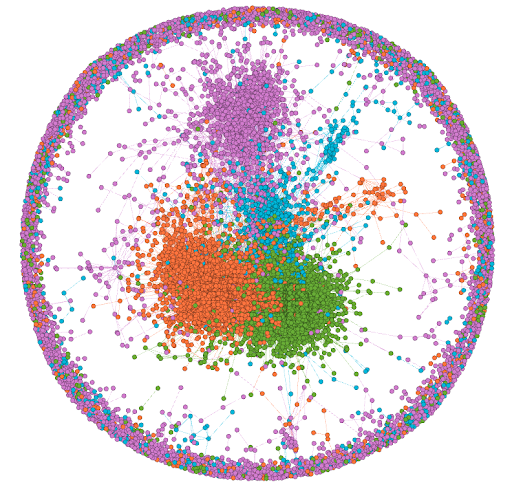
\includegraphics[scale=0.3] {wos_pic.png}}
    \caption{Large WoS network, Blue=ML Accelerators, Purple=Edge ML, Green=Neuromorphic Computing, Orange=Spiking Neural Network.}
    \label{fig}
\end{figure}

After applying these operations, the total number of nodes increases from 2,605 to 9,605 after removing 
unusable nodes. This graph also has 52,945 edges and 6,821 features, from applying the 
same methods of keyword extraction. When increasing the size of the dataset, we were also 
met with a class imbalance - there were far fewer papers in ML Accelerators in the WoS database, 
less than two thousand papers, while the other categories had over five thousand papers each. 
In this regard, we can infer that ML accelerators are less popular (or at least less explored) 
than other papers. However, since WoS is our only source of data, this could also result from 
a lack of these papers in the Web of Science database. Since class imbalances can also impact 
performance on ML models, this also acts as a limitation on the GNN models in use. \par

Recognizing that the number of features is nearly double that of any of the given datasets, 
this can also lead to excessive computation time and increased bias in the results from 
features that supply noise in the machine learning models. So, we then apply principal 
component analysis (PCA) to these features to select the features that best describe the 
classifications and links between each node. Here, we apply PCA with an explained variance 
of 80\% to provide a sufficient level of specificity without overfitting the data, 
reducing the number of features to 760. \par

Following this, we also update the characteristics of our graph, producing an average 
degree of 11.09, an average clustering coefficient of 0.158, and a diameter of 18. 
From the differences in these datasets, we see that the average degree of our dataset 
is much higher than the given datasets. However, the clustering coefficient and diameter 
of the dataset are comparable to those of other datasets. These metrics are compared to 
the other datasets in Table 1 below. \par 

From this table, we can see differences among the datasets explored in this paper, 
revealing the structural properties of these different graphs. Primarily, there are 
many more edges in the updated WoS compared to the other datasets, resulting in a much 
higher average degree for the updated dataset. However, the clustering coefficient for 
our dataset is still comparable to other datasets, implying that the field of machine 
learning hardware tends to have a significant number of citations, but a similar number 
of these papers forming a well-defined cluster. While Cora and CiteSeer are most similar 
to the WoS database in terms of content, both relating to machine learning, the graph 
characteristics of WoS are most similar to PubMed, with a higher degree and lower 
clustering coefficient. However, another limitation of utilizing WoS as our primary 
database is that it is unclear whether these characteristics arise as a quality of 
the database or as a characteristic of the field of ML hardware in general. \par

\begin{table}[htbp]
    \caption{Citation Network Characteristics}
    \begin{center}
        \begin{tabular}{|c|cccccc|}
        \hline
        % \textbf{Table}&\multicolumn{6}{|c|}{\textbf{Table Column Head}} \\
        % \cline{1-4} 
        \textbf{} & \textbf{\textit{Nodes}} & \textbf{\textit{Edges}} & \textbf{\textit{Features}} &
        \textbf{\textit{Degree}} & \textbf{\textit{CC$^{\mathrm{a}}$}} & \textbf{\textit{MD$^{\mathrm{b}}$}} \\
        \hline
        \textbf{\textit{Cora}} & 
        2708& 5429& 1433& 3.89807& 0.24067& 19 \\
        \textbf{\textit{CiteSeer}} & 
        3312& 4660& 3704& 2.81400& 0.14255& 28 \\
        \textbf{\textit{Pubmed}} & 
        19717& 44348& 500& 4.49632& 0.06017& 18 \\
        \textbf{\textit{Small WoS}} & 
        2605& 6600& 4134& 5.06717& 0.13529& 16 \\
        \textbf{\textit{Large WoS}} & 
        2605& 6600& 4134& 5.06717& 0.13529& 16 \\
        \hline
        \end{tabular}
        \label{tab1}
        {$^{\mathrm{a}}$Clustering Coefficient.}
        {$^{\mathrm{b}}$Maximum Diameter.}
    \end{center}
\end{table}

Before you begin to format your paper, first write and save the content as a 
separate text file. Complete all content and organizational editing before 
formatting. Please note sections \ref{AA}--\ref{SCM} below for more information on 
proofreading, spelling and grammar.

Keep your text and graphic files separate until after the text has been 
formatted and styled. Do not number text heads---{\LaTeX} will do that 
for you.

\subsection{Abbreviations and Acronyms}\label{AA}
Define abbreviations and acronyms the first time they are used in the text, 
even after they have been defined in the abstract. Abbreviations such as 
IEEE, SI, MKS, CGS, ac, dc, and rms do not have to be defined. Do not use 
abbreviations in the title or heads unless they are unavoidable.

\subsection{Units}
\begin{itemize}
\item Use either SI (MKS) or CGS as primary units. (SI units are encouraged.) English units may be used as secondary units (in parentheses). An exception would be the use of English units as identifiers in trade, such as ``3.5-inch disk drive''.
\item Avoid combining SI and CGS units, such as current in amperes and magnetic field in oersteds. This often leads to confusion because equations do not balance dimensionally. If you must use mixed units, clearly state the units for each quantity that you use in an equation.
\item Do not mix complete spellings and abbreviations of units: ``Wb/m\textsuperscript{2}'' or ``webers per square meter'', not ``webers/m\textsuperscript{2}''. Spell out units when they appear in text: ``. . . a few henries'', not ``. . . a few H''.
\item Use a zero before decimal points: ``0.25'', not ``.25''. Use ``cm\textsuperscript{3}'', not ``cc''.)
\end{itemize}

\subsection{Equations}
Number equations consecutively. To make your 
equations more compact, you may use the solidus (~/~), the exp function, or 
appropriate exponents. Italicize Roman symbols for quantities and variables, 
but not Greek symbols. Use a long dash rather than a hyphen for a minus 
sign. Punctuate equations with commas or periods when they are part of a 
sentence, as in:
\begin{equation}
a+b=\gamma\label{eq}
\end{equation}

Be sure that the 
symbols in your equation have been defined before or immediately following 
the equation. Use ``\eqref{eq}'', not ``Eq.~\eqref{eq}'' or ``equation \eqref{eq}'', except at 
the beginning of a sentence: ``Equation \eqref{eq} is . . .''

\subsection{\LaTeX-Specific Advice}

Please use ``soft'' (e.g., \verb|\eqref{Eq}|) cross references instead
of ``hard'' references (e.g., \verb|(1)|). That will make it possible
to combine sections, add equations, or change the order of figures or
citations without having to go through the file line by line.

Please don't use the \verb|{eqnarray}| equation environment. Use
\verb|{align}| or \verb|{IEEEeqnarray}| instead. The \verb|{eqnarray}|
environment leaves unsightly spaces around relation symbols.

Please note that the \verb|{subequations}| environment in {\LaTeX}
will increment the main equation counter even when there are no
equation numbers displayed. If you forget that, you might write an
article in which the equation numbers skip from (17) to (20), causing
the copy editors to wonder if you've discovered a new method of
counting.

{\BibTeX} does not work by magic. It doesn't get the bibliographic
data from thin air but from .bib files. If you use {\BibTeX} to produce a
bibliography you must send the .bib files. 

{\LaTeX} can't read your mind. If you assign the same label to a
subsubsection and a table, you might find that Table I has been cross
referenced as Table IV-B3. 

{\LaTeX} does not have precognitive abilities. If you put a
\verb|\label| command before the command that updates the counter it's
supposed to be using, the label will pick up the last counter to be
cross referenced instead. In particular, a \verb|\label| command
should not go before the caption of a figure or a table.

Do not use \verb|\nonumber| inside the \verb|{array}| environment. It
will not stop equation numbers inside \verb|{array}| (there won't be
any anyway) and it might stop a wanted equation number in the
surrounding equation.

\subsection{Some Common Mistakes}\label{SCM}
\begin{itemize}
\item The word ``data'' is plural, not singular.
\item The subscript for the permeability of vacuum $\mu_{0}$, and other common scientific constants, is zero with subscript formatting, not a lowercase letter ``o''.
\item In American English, commas, semicolons, periods, question and exclamation marks are located within quotation marks only when a complete thought or name is cited, such as a title or full quotation. When quotation marks are used, instead of a bold or italic typeface, to highlight a word or phrase, punctuation should appear outside of the quotation marks. A parenthetical phrase or statement at the end of a sentence is punctuated outside of the closing parenthesis (like this). (A parenthetical sentence is punctuated within the parentheses.)
\item A graph within a graph is an ``inset'', not an ``insert''. The word alternatively is preferred to the word ``alternately'' (unless you really mean something that alternates).
\item Do not use the word ``essentially'' to mean ``approximately'' or ``effectively''.
\item In your paper title, if the words ``that uses'' can accurately replace the word ``using'', capitalize the ``u''; if not, keep using lower-cased.
\item Be aware of the different meanings of the homophones ``affect'' and ``effect'', ``complement'' and ``compliment'', ``discreet'' and ``discrete'', ``principal'' and ``principle''.
\item Do not confuse ``imply'' and ``infer''.
\item The prefix ``non'' is not a word; it should be joined to the word it modifies, usually without a hyphen.
\item There is no period after the ``et'' in the Latin abbreviation ``et al.''.
\item The abbreviation ``i.e.'' means ``that is'', and the abbreviation ``e.g.'' means ``for example''.
\end{itemize}
An excellent style manual for science writers is \cite{b7}.

\subsection{Authors and Affiliations}
\textbf{The class file is designed for, but not limited to, six authors.} A 
minimum of one author is required for all conference articles. Author names 
should be listed starting from left to right and then moving down to the 
next line. This is the author sequence that will be used in future citations 
and by indexing services. Names should not be listed in columns nor group by 
affiliation. Please keep your affiliations as succinct as possible (for 
example, do not differentiate among departments of the same organization).

\subsection{Identify the Headings}
Headings, or heads, are organizational devices that guide the reader through 
your paper. There are two types: component heads and text heads.

Component heads identify the different components of your paper and are not 
topically subordinate to each other. Examples include Acknowledgments and 
References and, for these, the correct style to use is ``Heading 5''. Use 
``figure caption'' for your Figure captions, and ``table head'' for your 
table title. Run-in heads, such as ``Abstract'', will require you to apply a 
style (in this case, italic) in addition to the style provided by the drop 
down menu to differentiate the head from the text.

Text heads organize the topics on a relational, hierarchical basis. For 
example, the paper title is the primary text head because all subsequent 
material relates and elaborates on this one topic. If there are two or more 
sub-topics, the next level head (uppercase Roman numerals) should be used 
and, conversely, if there are not at least two sub-topics, then no subheads 
should be introduced.

\subsection{Figures and Tables}
\paragraph{Positioning Figures and Tables} Place figures and tables at the top and 
bottom of columns. Avoid placing them in the middle of columns. Large 
figures and tables may span across both columns. Figure captions should be 
below the figures; table heads should appear above the tables. Insert 
figures and tables after they are cited in the text. Use the abbreviation 
``Fig.~\ref{fig}'', even at the beginning of a sentence.

\begin{table}[htbp]
\caption{Table Type Styles}
\begin{center}
\begin{tabular}{|c|c|c|c|}
\hline
\textbf{Table}&\multicolumn{3}{|c|}{\textbf{Table Column Head}} \\
\cline{2-4} 
\textbf{Head} & \textbf{\textit{Table column subhead}}& \textbf{\textit{Subhead}}& \textbf{\textit{Subhead}} \\
\hline
copy& More table copy$^{\mathrm{a}}$& &  \\
\hline
\multicolumn{4}{l}{$^{\mathrm{a}}$Sample of a Table footnote.}
\end{tabular}
\label{tab1}
\end{center}
\end{table}

\begin{figure}[htbp]
\centerline{
\includegraphics{fig1.png}}
\caption{Example of a figure caption.}
\label{fig}
\end{figure}

Figure Labels: Use 8 point Times New Roman for Figure labels. Use words 
rather than symbols or abbreviations when writing Figure axis labels to 
avoid confusing the reader. As an example, write the quantity 
``Magnetization'', or ``Magnetization, M'', not just ``M''. If including 
units in the label, present them within parentheses. Do not label axes only 
with units. In the example, write ``Magnetization (A/m)'' or ``Magnetization 
\{A[m(1)]\}'', not just ``A/m''. Do not label axes with a ratio of 
quantities and units. For example, write ``Temperature (K)'', not 
``Temperature/K''.

\section*{Acknowledgment}

The preferred spelling of the word ``acknowledgment'' in America is without 
an ``e'' after the ``g''. Avoid the stilted expression ``one of us (R. B. 
G.) thanks $\ldots$''. Instead, try ``R. B. G. thanks$\ldots$''. Put sponsor 
acknowledgments in the unnumbered footnote on the first page.

\section*{References}

Please number citations consecutively within brackets \cite{b1}. The 
sentence punctuation follows the bracket \cite{b2}. Refer simply to the reference 
number, as in \cite{b3}---do not use ``Ref. \cite{b3}'' or ``reference \cite{b3}'' except at 
the beginning of a sentence: ``Reference \cite{b3} was the first $\ldots$''

Number footnotes separately in superscripts. Place the actual footnote at 
the bottom of the column in which it was cited. Do not put footnotes in the 
abstract or reference list. Use letters for table footnotes.

Unless there are six authors or more give all authors' names; do not use 
``et al.''. Papers that have not been published, even if they have been 
submitted for publication, should be cited as ``unpublished'' \cite{b4}. Papers 
that have been accepted for publication should be cited as ``in press'' \cite{b5}. 
Capitalize only the first word in a paper title, except for proper nouns and 
element symbols.

For papers published in translation journals, please give the English 
citation first, followed by the original foreign-language citation \cite{b6}.

\begin{thebibliography}{00}
\bibitem{b1} G. Eason, B. Noble, and I. N. Sneddon, ``On certain integrals of Lipschitz-Hankel type involving products of Bessel functions,'' Phil. Trans. Roy. Soc. London, vol. A247, pp. 529--551, April 1955.
\bibitem{b2} J. Clerk Maxwell, A Treatise on Electricity and Magnetism, 3rd ed., vol. 2. Oxford: Clarendon, 1892, pp.68--73.
\bibitem{b3} I. S. Jacobs and C. P. Bean, ``Fine particles, thin films and exchange anisotropy,'' in Magnetism, vol. III, G. T. Rado and H. Suhl, Eds. New York: Academic, 1963, pp. 271--350.
\bibitem{b4} K. Elissa, ``Title of paper if known,'' unpublished.
\bibitem{b5} R. Nicole, ``Title of paper with only first word capitalized,'' J. Name Stand. Abbrev., in press.
\bibitem{b6} Y. Yorozu, M. Hirano, K. Oka, and Y. Tagawa, ``Electron spectroscopy studies on magneto-optical media and plastic substrate interface,'' IEEE Transl. J. Magn. Japan, vol. 2, pp. 740--741, August 1987 [Digests 9th Annual Conf. Magnetics Japan, p. 301, 1982].
\bibitem{b7} M. Young, The Technical Writer's Handbook. Mill Valley, CA: University Science, 1989.
\end{thebibliography}
\vspace{12pt}
\color{red}
IEEE conference templates contain guidance text for composing and formatting conference papers. Please ensure that all template text is removed from your conference paper prior to submission to the conference. Failure to remove the template text from your paper may result in your paper not being published.

\end{document}
